\textbf{\large\color{orange}Zadanie 7.} Grassmannian $Gr_{\C}(k, n)$ ma pewien podział na komórki, który możemy opisać za pomocą szufladek i groszków. Rozważmy $n$ szufladek, w których umieszczać będziemy $k$ groszków, co najwyżej po jednym w danej szufladzie. Takie rozmieszczenie groszków reprezentuje zbiór $k$-wymiarowych podprzestrzeni $\C^n$. Kolejne $l$ szufladek od lewej reprezentuje podprzestrzeń $\C^n$ rozpiętą przez pierwsze $l$ wektorów bazowych $e_1, e_2,..., e_l$, a liczba groszków leżących w $l$ pierwszych $l$ szufladkach to wymiar przekroju $k$-wymiarowej podprzestrzeni z tego zbioru z podprzestrzenią rozpiętą przez $e_1,..., e_l$.
\begin{enumerate}[label=(\alph*)]
  \item Pokaż, że konkretne rozmieszczenie groszków w szufladach reprezentuje przestrzeń $k$-wymiarowych podprzestrzeni $\C^n$ izomorficzna z $\C^m$, gdzie $m$ to liczba przesunięć groszków w lewo o jedną szufladkę dopóki to możliwe.
  \item Przestrzeń $\C^m$ z poprzedniego podpunktu to otwarta komórka wspomnianego rozkładu. Komórka odpowiadająca rozmieszczeniu groszków $A$ zawiera się w
domknięcu komórki odpowiadającej rozmieszczeniu $B$, gdy $A$ można otrzymać z $B$ poprzez kolejne przesunięcia groszków w lewo o jedną szufladkę.
Domknięcie komórki odpowiadającej rozmieszczeniu $A$ nazywamy $(A)$ rozmaitością Schuberta. Policz charakterystykę Eulera rozmaitości Schuberta.
Policz charakterystykę Eulera $Gr_{\C}(k, n)$ zliczając te komórki
\end{enumerate}

\dotfill 

\begin{enumerate}[label=\textbf{(\alph*)}]
  \item Zacznijmy od rozmieszczenia groszków tak, że nie możemy już żadnego przesunąć w lewo.
    \begin{center}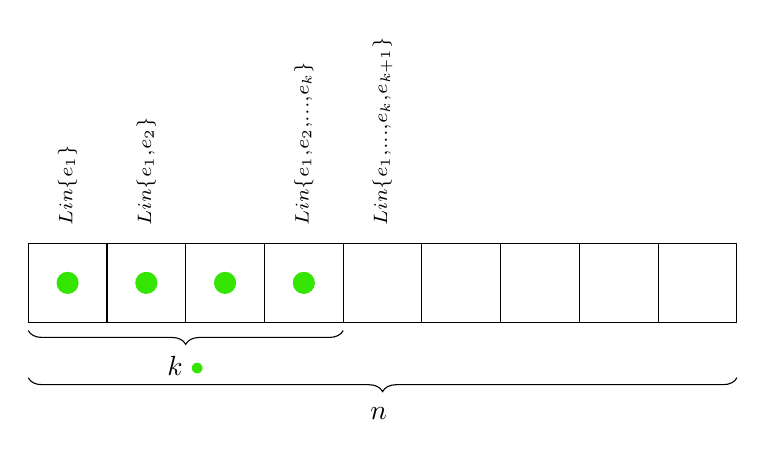
\begin{tikzpicture}
      \draw (1,0)--(10, 0);
      \draw (1, -1)--(10, -1);
      \foreach \i in {1,..., 10} \draw (\i, 0)--(\i, -1);
      \foreach \i in {1,...,4} \fill[green!80!orange] (\i+0.5, -0.5) circle (4pt);


      \draw[decorate,decoration={brace,amplitude=5pt,mirror,raise=4ex}] (1, -0.5)--(5, -0.5) node [midway, yshift=-3em] {$k\;\color{green!80!orange}\bullet$};
      \draw[decorate,decoration={brace,amplitude=5pt,mirror,raise=4ex}] (1, -1.1)--(10, -1.1) node [midway, yshift=-3em] {$n\;\square$};

      \node[rotate=90, anchor=west] at (1.5, 0.1) {$\scriptstyle Lin\{e_1\}$};
      \node[rotate=90, anchor=west] at (2.5, 0.1) {$\scriptstyle Lin\{e_1, e_2\}$};
      \node[rotate=90, anchor=west] at (4.5, 0.1) {$\scriptstyle Lin\{e_1, e_2, ..., e_k\}$};
      \node[rotate=90, anchor=west] at (5.5, 0.1) {$\scriptstyle Lin\{e_1, ..., e_k, e_{k+1}\}$};
    \end{tikzpicture}\end{center}

    To znaczy, że podprzestrzenie które są kodowane przez to ustawienie groszków kroją się niepusta z podprzestrzenią rozpinaną przez pierwszy wektor bazowy $e_1$, z podprzestrzenią rozpiętą przez dwa pierwsze wektory bazowe $e_1$, $e_2$ i tak dalej. W takim razie, typowa podprzestrzeń reprezentowana przez takie ustawienie jest generowana przez wektory
    \begin{align*}
      &e_1\\ 
      &a_1^1e_1+e_2\\ 
      &...\\ 
      &a_1^ke_1+a_2^ke_2+...+e_k
    \end{align*}
    Interesuje nas przestrzeń rozpinana przez takie wektory, więc w $i$-tym wektorze możemy usunąć część przychodzącą z $j<i$ wektorami. W ten sposób dostaniemy przestrzeń rozpiętą przez $e_1, e_2, ...,e_k$. Nie mamy żadnego parametru, więc jest to izomorficzne z punktem, czyli z $\C^0$.

    Załóżmy, że mamy $k$ groszków umieszczonych odpowiednio w szufladkach o numerze $m_1$, $m_2$, ..., $m_k$. 
    \begin{center}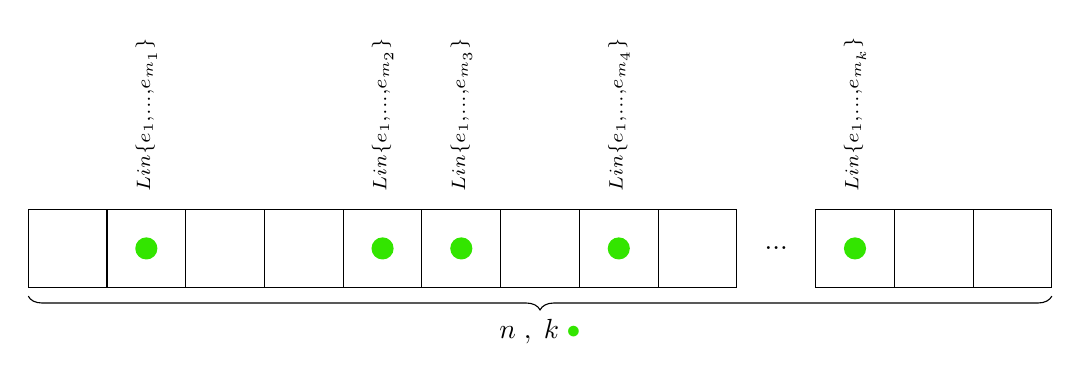
\begin{tikzpicture}
      \draw (1,0)--(10, 0);
      \draw (1, -1)--(10, -1);
      \foreach \i in {1,..., 10} \draw (\i, 0)--(\i, -1);

      \fill[green!80!orange] (2.5, -0.5) circle (4pt);
      \fill[green!80!orange] (5.5, -0.5) circle (4pt);
      \fill[green!80!orange] (6.5, -0.5) circle (4pt);
      \fill[green!80!orange] (8.5, -0.5) circle (4pt);

      \draw[decorate,decoration={brace,amplitude=5pt,mirror,raise=4ex}] (1, -0.5)--(14, -0.5) node [midway, yshift=-3em] {$n\;\square,\;k\;\color{green!80!orange}\bullet$};

      \node[rotate=90, anchor=west] at (2.5, 0.1) {$\scriptstyle Lin\{e_1,..., e_{m_1}\}$};
      \node[rotate=90, anchor=west] at (5.5, 0.1) {$\scriptstyle Lin\{e_1,..., e_{m_2}\}$};
      \node[rotate=90, anchor=west] at (6.5, 0.1) {$\scriptstyle Lin\{e_1,..., e_{m_3}\}$};
      \node[rotate=90, anchor=west] at (8.5, 0.1) {$\scriptstyle Lin\{e_1,..., e_{m_4}\}$};
      
      \node at (10.5, -0.5) {...};
      \foreach \i in {1,..., 4} \draw (\i+10, 0)--(\i+10, -1);
      \draw (11, 0)--(14, 0);
      \draw (11, -1)--(14, -1);

      \fill[green!80!orange] (11.5, -0.5) circle (4pt);
      \node[rotate=90, anchor=west] at (11.5, 0.1) {$\scriptstyle Lin\{e_1,..., e_{m_k}\}$};
    \end{tikzpicture}\end{center}
    Dzięki pierwszemu groszkowi możemy do naszej $k$-wymiarowej podprzestrzeni $\C^n$ wybrać wektor
    $$a_1^{m_1}e_1+a_2^{m_1}e_2+...+e_{m_1}.$$
    Kolejny groszek, na $m_2> m_1$ miejscu pozwoli nam dołożyć wektor
    $$a_1^{m_2}e_1+a_2^{m_2}e_2+...+a_{m_1}^{m_2}+...+e_{m_2}.$$
    Ze współczynników pojawiających się przy kolejnych $e_i$ możemy stworzyć macierz
    $$
    \begin{bmatrix}
      a_1^{m_1} & a_2^{m_1} & ... & 1 & 0 & ... & 0 & ... & 0\\ 
      a_1^{m_2} & a_2^{m_2} & ... & a_{m_1}^{m_2} & ... & ... & 1 & 0 & ...\\ 
      \vdots & \vdots & \vdots & \vdots & \vdots\\ 
      a_1^{m_k} & a_2^{m_k} & ... & a_{m_1}^{m_k} & ... & ... & ... & ... & 1 
    \end{bmatrix}
    $$
    która ma $m_k$ kolumn i $k$ wierszy. Możemy skorzystać z algorytmu eliminacji Gaussa, by dostać w pierwszych $k$ kolumnach kwadratową macierz górnotrójkątną z $1$ na przekątnej. 

    W pierwszym wierszu zostaje nam $(m_1-1)$ zmiennych, w drugim wierszu mamy $(m_2-2)$ nowych zmiennych i tak dalej. Sumarycznie dostajemy
    $$\sum_{i=1}^k(m_i-i)$$
    parametrów w takiej macierzy, co jest równe ilości potencjalnych przesunięć groszków: $i$-ty groszek może przejść przez co najwyżej $(m_i-i)$ szufladek, niekoniecznie za jednym zamachem.

    Pokazaliśmy, że jeśli możemy dokonać $m$ przesunięć groszków, to takie ustawienie możemy zapisać jako przestrzeń liniową przy pomocy $m$ parametrów. Jest to więc przestrzeń izomorficzna z $\C^m$.

  \item Przejścia od dowolnego ułożenia groszków $A$ do ułożenia, gdzie nie możemy już wykonać ruchów możemy przedstawić jako graf, gdzie wierzchołki to ułożenia pośrednie:
    \begin{center}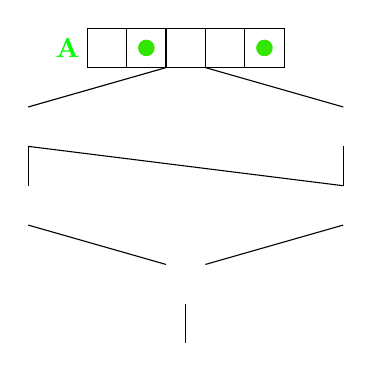
\begin{tikzpicture}
      \draw (0, 0)--(2.5, 0);
      \draw (0, -0.5)--(2.5, -0.5);
      \foreach \i in {0, 1, 2, 3, 4, 5} \draw (\i/2, 0)--(\i/2, -0.5);
      \foreach \j in {1, 4} \fill[green!80!orange] (\j/2+0.25, -0.25) circle (3pt);

      \node at (-0.25, -0.25) {\textbf{\color{green}A}};

      \groszki{(-2, -1)}{1, 3}
      \groszki{(2, -1)}{0, 4}

      \groszki{(-2, -2)}{1, 2}
      \groszki{(2, -2)}{0, 3}

      \groszki{(0, -3)}{0, 2}
      \groszki{(0, -4)}{0,1}

      \draw (1, -0.5)--(-0.75, -1);
      \draw (1.5, -0.5)--(2+1.25, -1);

      \draw (-0.75, -1.5)--(-0.75, -2);
      \draw (-0.75, -1.5)--(2+1.25, -2);
      \draw (3.25, -1.5)--(3.25, -2);

      \draw (3.25, -2.5)--(1.5, -3);
      \draw (-0.75, -2.5)--(1, -3);

      \draw (1.25, -3.5)--(1.25, -4);
    \end{tikzpicture}\end{center}

    Przez $a_i$ oznaczmy ilość wierzchołków w wierszu $i$, liczonym od dołu. Najniższy wiersz liczymy jako wiersz zerowy. Charakterystyka Eulera $(A)$, jeśli ustawienie $A$ jest na wierszu $m$ od dołu, wyniesie
    $$\chi((A))=\sum_{i=0}^{m}(-1)^i\cdot a_i.$$
    Czyli dla rysunku wyżej, $\chi((A))=1-1+2-2+1=1$.

    Wprost najłatwiej jest wyliczyć charakterystykę Eulera $(A)$ dla $A$ z małą liczbą przesunięć. Np. dla ustawienia trywialnego, tzn. 
    \begin{center}\begin{tikzpicture}\groszki{(0,0)}{0,1,2}\end{tikzpicture}\end{center} 
    charakterystyka Eulera rozmaitości Schuberta to $1$.

    Jeśli możemy wykonać tylko jeden ruch, tzn. mamy ustawienie
    \begin{center}\begin{tikzpicture}\groszki{(0,0)}{0,1,3}\end{tikzpicture}\end{center} 
    to rozmaitość Schuberta ma charakterystykę $0$. Ustawienie gdzie możemy wykonać dwa ruchy to z kolei $1$, gdyż po pierwszym ruchu wylądujemy z powrotem w przypadku narysowanym wyżej. Będziemy więc mieli trzy wiersze w grafie, każdy mający tylko jeden element.

    Jeśli z $A$ możemy wykonać $3$ ruchy, mamy już o wiele bardziej skomplikowaną pozycję. Jeśli $A$ ma ostatni groszek oddalony o $3$ szufladki od pozostałych, to dostajemy prosty graf
    \begin{center}\begin{tikzpicture}
      \groszki{(0,0)}{0,4}
      \groszki{(3, 0)}{0, 3}
      \groszki {(6, 0)} {0, 2}
      \groszki {(9, 0)} {0, 1}
    \end{tikzpicture}\end{center}
    i charakterystykę Eulera $0$. Możemy też mieć ustawienie
    \begin{center}\begin{tikzpicture}
      \groszki{(0,0)}{1, 3}
    \end{tikzpicture}\end{center}
    wtedy pierwszy ruch wykonujemy na dwa sposoby - charakterystyka Eulera wyniesie 
    $$\chi=-1+2\cdot 1-1+1=1$$
    Ostatnim możliwym ustawieniem skrajnie prawych groszków na $3$ ruchy jest
    \begin{center}\begin{tikzpicture}
      \groszki{(0,0)}{1,2,3} 
      \groszki{(3,0)}{0,2,3}
      \groszki{(6, 0)}{0,1,3}
      \groszki{(9, 0)}{0,1,2}
    \end{tikzpicture}\end{center}
    z charakterystyką Eulera równą $0$.

    Charakterystykę Eulera całego Grassmanianu liczymy dodając charakterystykę Eulera kolejnych komórek Schuberta:
    $$\chi(Gr_{\C}(k,n))=\sum_{\substack{(A):A\in Gr}}\chi((A))=\binom{n}{k}$$
    gdyż jest to ilość wierzchołków w grafie kolejnych przejść od ustawienia wszystkich $k$ groszków skrajnie po prawej stronie do ustawienia skrajnie po lewej stronie.





%    W tym podpunkcie pytamy tak naprawdę, na ile możliwości możemy dojść do "trywialnego" ułożenia zaczynając w ułożeniu $A$. Każde ułożenie pośrednie będziemy ewaluować $1$ lub $(-1)$ w zależności od tego, czy jest izomorficzne z $\C^{2k}$ (wtedy $+1$) czy z $\C^{2k+1}$ (wówczas $-1$).
%
%    Ułożenie $k$ groszków w $n$ szufladkach jest jednoznacznie wyznaczane przez położenia $m_1<m_2<...<m_k$ kolejnych groszków. Z takiego ułożenia możemy otrzymać inne przez przesuwanie w lewo dowolne ustawienie, w której na pozycjach $>m_{k-1}$ jest co najwyżej jeden groszek, na pozycjach $>m_{k-2}$ - co najwyżej dwa groszki i tak dalej.
%
%    Możemy ułożyć $m_k$ zer w ciągu i $k$ spomiędzy nich zamienić na jedynki, symbolujące położenie groszków, i zastanawiać się, które ułożenia są niedozwolone. $k$ jedynki możemy wybrać bez restrykcji na $\binom{m_k}{k}$ sposobów. 
%
%    Niedozwolone ułożenia posiadają co najmniej $(i+1)$ groszków na pozycjach $m_{k-i}$. Takich ułożeń jest $\binom{m_k-m_{k-i}}{i+1}\cdot\binom{m_k-i-1}{k-i-1}$. Dostajemy z zasady włączeń i wyłączeń wzór
%    $$\sum_{i=0}(-1)^i\binom{m_k-m_{k-i}}{i+1}\cdot\binom{m_k-i-1}{k-i-1}$$
%    na ilość możliwych przesunięć w lewo groszków z ustawienia $m_1<m_2<...<m_k$.
%
%    Teoretycznie charakterystyka Eulera powinna wyjść $\binom{n}{k}$, czyli na ile sposobów możemy ułożyć $k$ groszków w $n$ szufladkach. Jest to równe ilości wierzchołków w grafie, który od $k$ groszków ustawionych skrajnie po prawej stronie przechodzi do $k$ groszków ustawionych skrajnie po lewej stronie na wszystkie możliwe sposoby.
\end{enumerate}
